In this section, we explore the synergies between sequence transformation and completion---
and investigate \emph{improving} a sequence, such as trajectories in a sequential decision process, along some metric, such as a reward function.
Here, we use an LLM to generate new sequences $x^N$ conditioned on previous sequences $(x^{1}, \ \ldots, \ x^{N-1})$, which can represent previous iterations of the same sequence (or policy it represents). The improvement can also be return-conditioned, given a reward function $r(\cdot)$. By inserting as the first token(s) of each sequence its corresponding total reward $x = (r(x), s_1\ , \ ...,\ s_k)$, we can prompt the model to conditionally ``improve'' by ``just asking'' \cite{jang2021just} for a higher reward than those seen in-context (\ie prompting LLMs to act as Decision Transformers \cite{chen2021decision}). New ``rollouts'' can yield new reward labels that then replace the original desired rewards with actual rewards.
Iteratively performing this inference and accumulating trajectories may jointly use the model's general notion of pattern transformation and extrapolation to perform improvement of sequences, which can be represented by numeric or symbolic tokens.
Note that there are practical considerations, \eg depending on the task or model, not all sequences can fit in context, so options could be to keep the most recent, or the ones with the highest rewards if available (see Appendix for more discussion).
In this section, we perform a series of targeted experiments on simple tasks, aiming to explore the possibility of using LLMs for sequence improvement in trajectory and policy optimization.

\begin{wrapfigure}{r}{0.4\textwidth}
    \vspace{-1.3em}
    \centering
    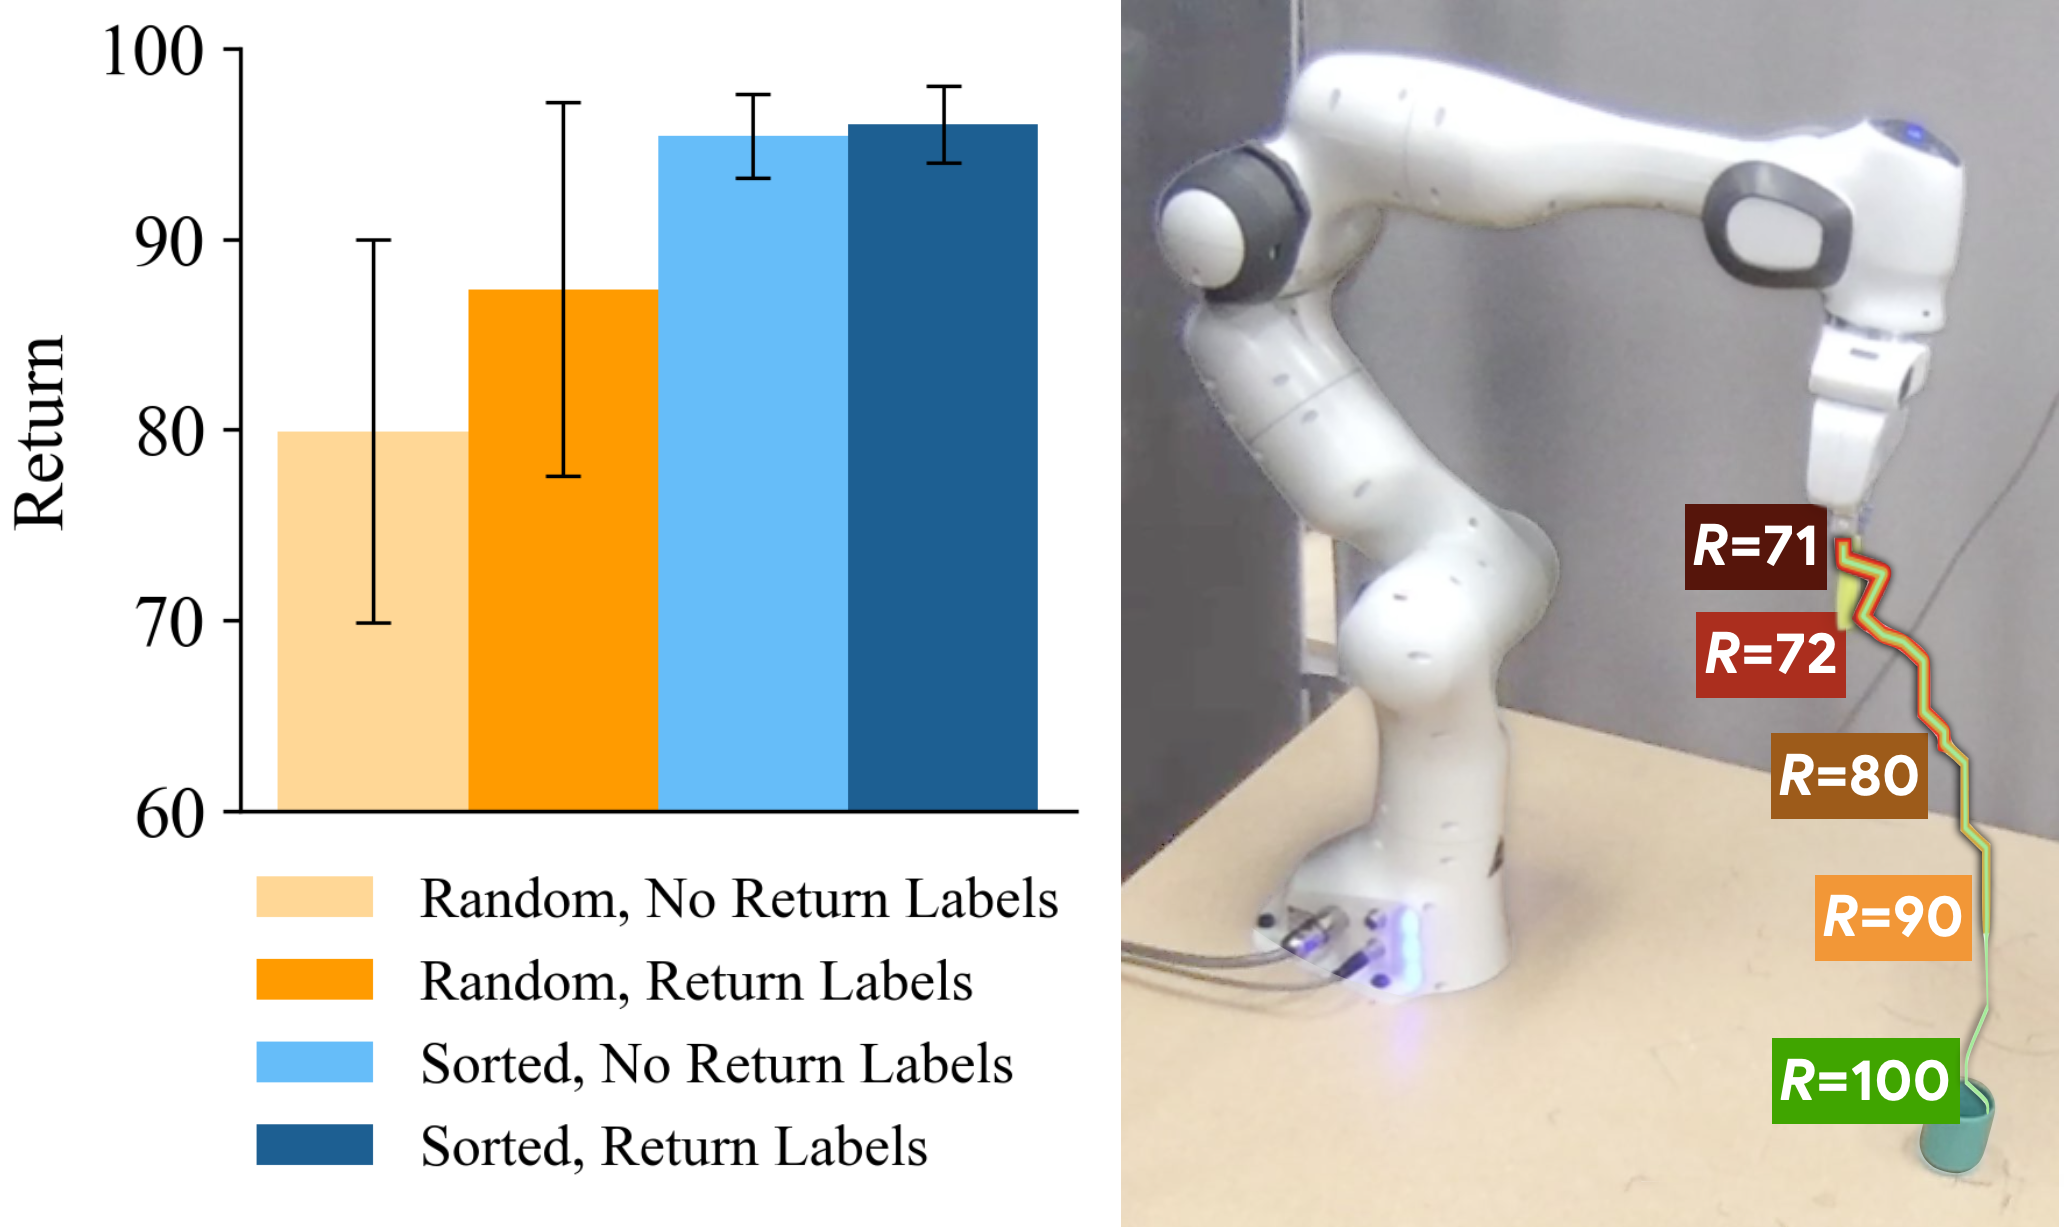
\includegraphics[width=1.0\textwidth]{figures/marker_in_cup_rewards_and_figure_v3.png}
    \caption{\small
    LLM agents can generate new trajectories with increasing returns for a \textit{Marker in Cup} task (right). Performance varies with different ways of building the context (left).
    \vspace{-1em}
    }
    \label{fig:marker_in_cup_rewards}
    \vspace{-0.7em}
\end{wrapfigure}

\textbf{Extrapolating simple meta-patterns among trajectories.}
Sequence improvement with LLMs enables a simple form of trajectory optimization
for a \textit{Marker in Cup} task on a Franka Panda robot, where we define the prefixed reward of a trajectory to be the negative distance between the final end-effector position and the cup (normalized between 0--100), and initialize the context with a collection of trajectories (stopping at 20\%, 40\%, 60\%, and 80\% of the way to the cup), delimited by newlines and prefixed by rewards (ranging roughly from 70-90; see Appendix). For this task, we represent trajectories as sequences of Cartesian positions, each dimension normalized between 0--100. We find that text-davinci-003, to an extent, is able to generalize the pattern and generate a trajectory that achieves a reward $>90$. For this extrapolation to occur, we observe that meta-patterns in the context are crucial: in \cref{fig:marker_in_cup_rewards} (left), we compare the average reward achieved by text-davinci-003 over 11 trials (each with a different goal position) given contexts with different trajectory orderings (sorted by reward, randomly permuted, or with/without reward annotations). \looseness=-1

\begin{wrapfigure}{r}{0.23\textwidth}
    \vspace{-1.3em}
    \centering
    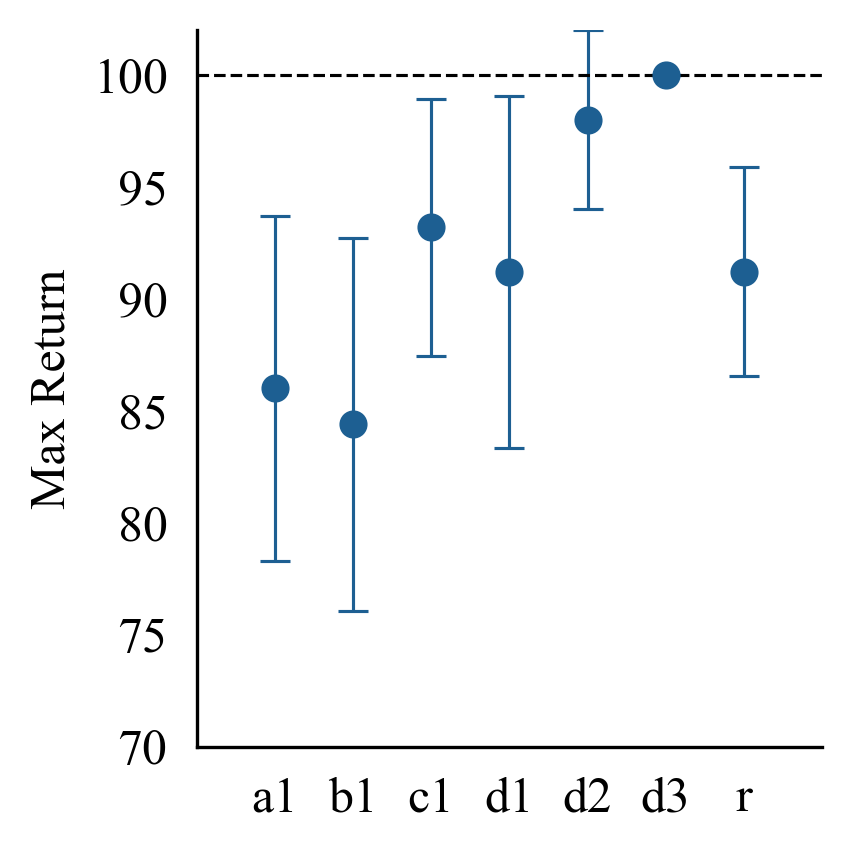
\includegraphics[width=\textwidth]{figures/grid-return.png}
    \caption{\small
    Average max return for LLM agents a1-d3 on \textit{Grid} compared to random exploration (r).
    \vspace{-1em}
    }
    \label{fig:grid_return}
    \vspace{-0.7em}
\end{wrapfigure}

\textbf{Sampling higher-reward trajectories online.} While LLMs can extrapolate from trajectories that exhibit clear meta-patterns among them, we find that this ability is more limited for less trivial setups. Consider a simple $9\times9$ \textit{Grid} navigation environment with a random goal position and a fixed starting position at the grid center. Episodes terminate after 20 timesteps, and the return is based on the distance from the agent to the goal at the final time step. This environment is inspired by the Dark Room environment from \cite{laskin2022context} but with a continuous reward function, reducing the exploration challenge.
The agent may take actions (1-5) corresponding to moving right, up, left, down, and no-op. We initialize the context buffer with 20 trajectories of agent grid positions generated by a random policy, sorted by total cumulative rewards. These trajectories exhibit a more complicated meta-pattern than in the \textit{Marker in Cup} task; we do not find that LLMs can generate trajectories of higher reward immediately. With that said, we can consider an iterative, \textit{online }setting, in which the LLM acts as an agent that interacts with the environment in a closed-loop. The context consists of the highest reward trajectories in sorted order, appended with a higher reward than was seen in the context, plus states and actions from the current partial trajectory (see Appendix). Once an episode terminates, its trajectory is relabeled with the reward achieved, and inserted into the context at the appropriate position. In \cref{fig:grid_return}, we plot the maximum return attained by a1-d3 over 50 episodes, compared to random exploration, averaged over 5 trials. We find that a1-d1 tend to sometimes ``exploit'' the suboptimal behaviors represented in the context (which initially contains trajectories with rewards ranging from 6-78), whereas d3 can consistently find a solution to \textit{Grid} within 50 episodes.

\begin{wrapfigure}{t}{0.5\textwidth}
    \vspace{-1.5em}
    \centering
    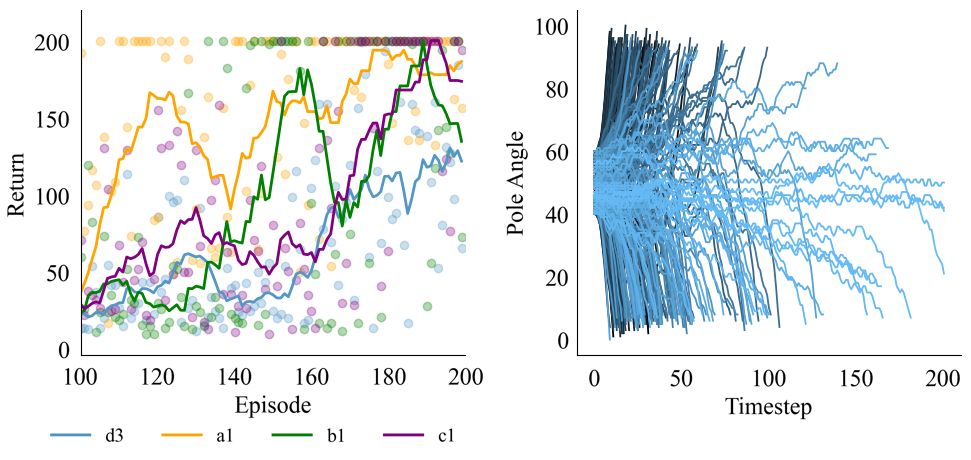
\includegraphics[width=\textwidth]{figures/cartpole_rewards_v2.png}
    \caption{\small
    Different LLM agents (d3 - c1) on average can improve trajectories (total rewards) with more \textit{CartPole} episodes (left), and discovers ``oscillatory behaviors'' (right) to keep the CartPole upright (later episodes are brighter).
    \vspace{-1em}
    }
    \label{fig:cartpole}
    \vspace{-0.5em}
\end{wrapfigure}

\textbf{Discovering a simple \textit{CartPole} controller.} We show that using LLMs as agents in an online, closed-loop setting can discover a simple controller for \textit{CartPole} (where observations consist of pole angle and velocity, normalized to 0--100, actions are 1 (left) and 2 (right), maximum horizon is 200). \cref{fig:cartpole} (left) shows that  return (number of steps the CartPole is kept upright) improves on average across various LLMs over 100 episodes (where the first 100 are generated by random exploration). \cref{fig:cartpole} (right) shows the evolution of trajectories over episodes of d3, demonstrating that it discovers oscillatory behaviors to keep the CartPole upright.


\begin{wrapfigure}{r}{0.5\textwidth}
    \vspace{-1em}
    \centering
    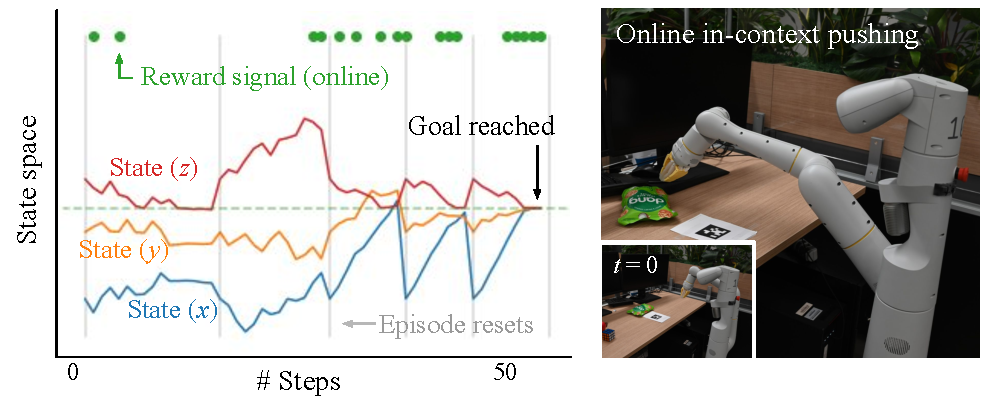
\includegraphics[width=\textwidth]{figures/clicker-training-v3.pdf}
    \caption{\small{LLMs can in-context react to sparse reward signals online to encourage an end effector to reach a desired goal.
    \vspace{-1em}  %
    }}
    \label{fig:clicker}
    \vspace{-0.8em}  %
\end{wrapfigure}

\textbf{Online human-guided trajectory optimization.} LLMs can also react to sparse binary reward signals (\eg subjectively provided by a human) to adjust trajectories online. This is analogous to an implementation of ``clicker training'' \cite{kaplan2002robotic,chiandetti2016can} used for training dogs, but instead applied to robots.
In this setup, at every time step (2s), the robot executes an action corresponding to a movement of its end-effector in a particular direction. The human observes the action and chooses whether to give a reward (\ie by using the clicker) to encourage or discourage similar behaviors. Episodes reset after 30 seconds, and the first two episodes are generated by random exploration. The (\textit{reward}, \textit{state}, \textit{action}) tuples are added as in-context examples (with negative examples followed by positives, and an equal number of each) to generate the next action based on the current state. An example context format is given in the Appendix. As shown in \cref{fig:clicker}, applying LLMs' sequence improvement capabilities in this way enables a human to guide the robot to push an object.